%Numero de paginas en dvi =
\documentclass[]{rmf-d}
\usepackage{nopageno,rmfbib,multicol,times,epsf,amsmath,amssymb}
\usepackage[latin1]{inputenc}
\usepackage[spanish]{babel}
\usepackage[]{caption2}
\usepackage{graphicx}
\usepackage{float}

\def\rmfcornisa{Informaci\'on cu\'antica \hfill\rmf\ {\bf 48} (6) ???--??? % Suponiendo Vol 48 num 6 y area ENSEÑANZA
\hfill Marzo 2019}
\newcommand{\ssc}{\scriptscriptstyle}

\def\rmfcintilla{{\it Rev.\ Mex.\ F\'{\i}s.\/} {\bf 48} (6) (2003) ???--???}
\clearpage \rmfcaptionstyle \pagestyle{myheadings}
\setcounter{page}{1} \markboth{Alejandro.}
{T\'itulo del trabajo}
\begin{document}
	\title{Inteligencia artificial para encontrar la soluci\'on num\'rica de la ecuaci\'on de Schr\"odinger
	\vspace{-6pt}}

	\author{Alejandro Grcía.}
	\address{TNM\\
		TESOEM}

	%\author{Nombre del Autor}
	%\address{Dependencia y direcci\'on}

	\maketitle \recibido{ de  de }{ de  de \vspace{-12pt}} % Fecha de recibido y aceptado (ej. 3 de abril de 2002)

	% En ingles va primero el abstract y luego el resumen

	\begin{resumen}
		\input{content/resumen}
	\end{resumen}
	\descript{ Incluir aqui los descriptores \vspace{-4pt}}
	\begin{abstract}
		\input{content/resumen}
	\end{abstract}
	\keys{Incluir aqui los Keywords \vspace{-4pt}} \pacs{Incluir aqui
	los numeros PACS \vspace{-4pt}}
	\begin{multicols}{2}
		\section{Introducci\'on}
			Una red neuronal artificial (RNA) es concebida como un
procesador paralelo y distribuido que consiste de un gran
n\'umero de unidades de c\'omputo, conocidas como neuronas.
La interconexi\'on masiva entre neuronas tiene como objetivo
almacenar informaci\'on que representa conocimiento
o experiencia. Esta informaci\'on se define a trav\'es de la fuerza de
interconexi\'on neuronal, o peso sin\'aptico. Las redes neuronales
tienen la capacidad de aproximar funciones. Con respecto
a la ecuaci\'on de Schr\"odinger una RNA se usa para describir
la funci\'on de onda de un sistema cu\'antico. El entrenamiento
de la RNA se lleva a cabo utilizando un proceso de aprendizaje
de tal manera que las entradas-salidas de la red satisfacen
la ecuaci\'on de Schr\"odinger. Se considera que las redes neuronales
artificiales tienen la capacidad de describir de forma
eficiente a una funci\'on propia, pero dada la gran cantidad de
m\'inimos existentes en el espacio de b\'usqueda se hace dif\'icil
encontrar la soluci\'on exacta. La respuesta de una red entrenada
depende considerablemente de los pesos iniciales independientemente
del proceso de aprendizaje utilizado.

Un algoritmo gen\'etico (AG) es una t\'ecnica de b\'usqueda
basada en estrategias evolutivas, se ha usado este tipo de
algoritmo para resolver problemas de optimizaci\'on en campos
como la qu\'imica, optimizaci\'on geom\'etrica de sistemas
rob\'oticos y mecatr\'onicos. La desventaja de un AG es su lenta
convergencia hacia la soluci\'on exacta. 

La idea es combinar una RNA y un AG con el fin de resolver
la ecuaci\'on de Schr\"odinger. La habilidad de las redes neuronales
para describir las entradas-salidas relacionadas con
conductas complejas puede ser utilizada para representar a las
funciones de onda excitadas de un sistema cu\'antico, mientras
que la ventaja de un AG con respecto a b\'usquedas globales
ayudar\'a a la RNA evitando una prematura convergencia durante
el proceso de aprendizaje.
		\section{Propuesta}
			\subsection{Red neuronal artificial}
Una red neuronal (RN) es un modelo constituido por un
n\'umero masivo de unidades de c\'omputo de dise\~no simple
conocidas como neuronas. La figura \ref{fig:neurona}  muestra un ejemplo
de una neurona.

\begin{figure}[H]
	\centering
	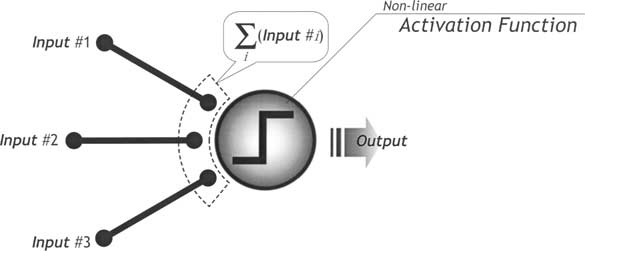
\includegraphics[width=5cm]{img/neurona.jpg}
	\caption{Modelo de unidad de c\'omputo simple, neurona.}
	\label{fig:neurona}
\end{figure}

Todas las se\~nales que ingresan a la neurona son sumadas,
al final la amplitud de la se\~nal de salida de la neurona se
determina por una funci\'on de activaci\'on no-lineal $\sigma(z)$. Aqu\'i
se hace uso de la siguiente ecuaci\'on: 
\begin{equation}
	\sigma(z)=\frac{1-e^{-kz}}{1+e^{-kz}}
\end{equation}

La figura \ref{fig:activa} considera $k=1$, conforme $k\rightarrow\infty$ la funci\'on
$\sigma(z)$ se comporta como una funci\'on escal\'on. Es conveniente
considerar a la funci\'on de activaci\'on con una inclinaci\'on
moderada con esto la respuesta de la red estar\'a dentro de un
rango de valores $\left[1-,1\right]\subset\Re$, lo anterior muestra la diferenciabilidad
de la red.

\begin{figure}[H]
	\centering
	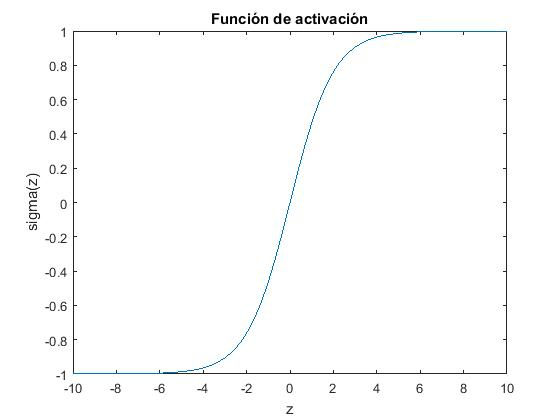
\includegraphics[width=5cm]{img/activa.jpg}
	\caption{Gr\'afica de  la funci\'on de activaci\'on.}
	\label{fig:activa}
\end{figure}

Se considera una RNA de tres capas cuya topolog\'ia se
muestra en la figura \ref{fig:percep}.  

\begin{figure}[H]
	\centering
	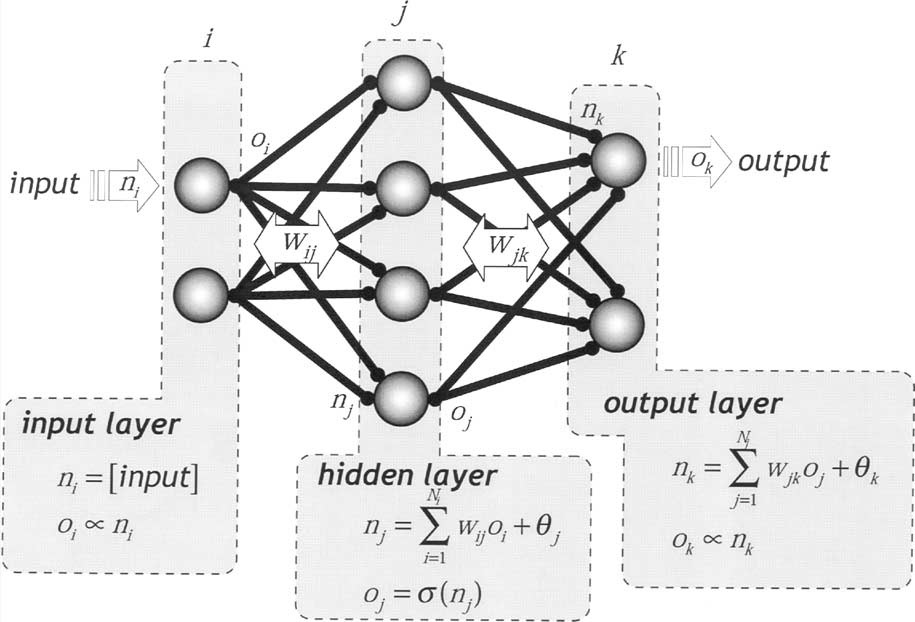
\includegraphics[width=5cm]{img/percep.jpg}
	\caption{Topolog\'ia de la RNA con capa de entrada, oculta y salida.}
	\label{fig:percep}
\end{figure}

Los indices $i$, $j$ y $k$ se asocian con las neuronas de la capa
de entrada, oculta y salida, respectivamente. Adem\'as, $n_i$ representa
la entrada de la $i$-\'esima neurona, y $o_i$ su correspondiente
salida. La entrada-salida propiedad de cada neurona
matem\'aticamente se expresa como: 

\begin{equation}
	o_i=\sigma(n_i)
	\label{entrada}
\end{equation}
\begin{equation}
	o_j=\sigma(n_j)
	\label{oculta}
\end{equation}
\begin{equation}
	o_k=\sigma(n_k)
	\label{salida}
\end{equation}

Las entradas a cada distinto tipo de neurona dependiendo
de la capa a la que pertenece, se expresa de siguiente forma:

\begin{equation}
	n_i=\text{est\'imulos ambientales de la RNA} \label{estimulo}
\end{equation}
\begin{equation}
	n_j=\sum^{N_i}_{i=1}w_{ij}o_i+\theta_j
\end{equation}
\begin{equation}
	n_k=\sum^{N_j}_{j=1}w_{jk}o_j+\theta_k
\end{equation}

$N_i$ y $N_j$ representan el n\'umero de unidades que forman
las capas de entrada y oculta respectivamente, mientras que
$w_{ij}$ es el peso sin\'aptico que determina la fuerza de conexi\'on
entre las neuronas $i$ y $j$. Por \'ultimo, el par\'ametro de umbral
relacionado con la neurona $j$ se representa por $\theta_j$.

La RNA representar\'a la funci\'on de onda, la funci\'on sigmoidal
solo se emplea en la capa oculta con el fin de suavizar
y moderar la respuesta de la red. La respuesta total por parte
de la red esta dada por:

\begin{equation}
	o_k=\sum^{N_j}_{j=1}w_{jk}\sigma(\sum^{N_i}_{i=1}w_{ij}n_i+\theta_j)+\theta_k
\end{equation}

Al derivar $o_k$ con respecto a los par\'ametros que definen
el comportamiento de la red se obtiene el siguiente conjunto
de ecuaciones:

\begin{equation}
	\frac{\partial o_k}{\partial w_{ij}}=w_{jk}\sigma' (n_j)n_i
\end{equation}
\begin{equation}
	\frac{\partial o_k}{\partial w_{jk}}=\sigma (n_j)\delta_{kk'}
\end{equation}
\begin{equation}
	\frac{\partial o_k}{\partial \theta_j}=w_{jk}\sigma' (n_j)
\end{equation}
\begin{equation}
	\frac{\partial o_k}{\partial \theta_k}=\delta_{kk'}
\end{equation}


Cada una de estas ecuaciones juega un papel importante
en el proceso de aprendizaje de la RNA. Esta informaci\'on
de razones de cambio indican las direcciones correctas para
ajustar los par\'ametros que permiten sintonizar la respuesta de
la red lo mas pr\'oxima posible a una respuesta deseada. Resta
considerar las derivadas de la salida de la red con respecto a
las entradas o est\'imulos recibidos por la red, en general estas
se expresan:

\begin{equation}
	\frac{\partial^\lambda o_k}{\partial n_i^\lambda}=\sum^{N_j}_{j=1}w_{jk}\sigma^\lambda(n_j)w_{ij}^\lambda
	\label{lamda}
\end{equation}

\subsection{Algoritmo gen\'etico}

Un algoritmo gen\'etico (AG) requiere para trabajar codificar
las variables a ser optimizadas. Estas variables forman
una cadena, idea correspondiente con el cromosoma en biolog\'ia.
Cada variable real se representa como una subcadena
binaria, parte de la cadena final o cromosoma.

El azar constituye el elemento conductor de la fuerza de
un AG que lo hace un optimizador eficiente. El operador mutaci\'on
es una fuente de azar en los algoritmos gen\'eticos cl\'asicos.
Una propuesta distinta conocida como micro-AG trata
de restablecer ocasionalmente la poblaci\'on en el proceso de
b\'usqueda global, por tal efecto se requiere de una poblaci\'on
peque\~na.

El AG comienza con la construcci\'on de una poblaci\'on
inicial aleatoria con una longitud de cromosoma dependiente
de la cantidad de par\'ametros a ser optimizados. El paso
siguiente consiste en evaluar a cada individuo de la poblaci\'on
con lo que se le asigna un valor de aptitud. La selecci\'on simula
el proceso de selecci\'on natural donde un individuo con alto
puntaje de aptitud se reproduce, y aquel individuo con puntajes
pobres es eliminado. Aqu\'i se considera la selecci\'on por
torneo, donde aleatoriamente se eligen dos individuos de la
poblaci\'on, sus puntajes de aptitud son comparados, aquel con
mayor valor se mantiene para la siguiente etapa, este proceso
se repite hasta tener un n\'umero considerable de individuos.

La poblaci\'on se actualiza por operaciones de apareamiento
y cruzamiento. La operaci\'on de cruzamiento lleva a cabo
el intercambio aleatorio de informaci\'on gen\'etica entre pares
de individuos para crear a sus descendientes. Se emplea cruzamiento
uniforme, en el cual se consideran diversos puntos
de cruzamiento determinados aleatoriamente en conjunci\'on
con sus respectivas posiciones en el cromosoma.

Por \'ultimo, en cada generaci\'on se verifica la convergencia
de la poblaci\'on. \'esta se mide por $D$ que define las diferencias
entre el individuo m\'as apto con el resto de los individuos
de la poblaci\'on. Se\~nal que la poblaci\'on evoluciona es que
$D\geq\epsilon\geq0.05$ en tal caso se pasa a la siguiente generaci\'on.
En otro caso se aplica elitismo, esto significa dejar al individuo
m\'as apto, y restablecer la poblaci\'on aleatoriamente.

\subsection{Mec\'anica cu\'antica}

Sinergia entre redes neuronales artificiales, algoritmo
gen\'eticos y mec\'anica cu\'antica. Un sistema cu\'antico
uno-dimensional es gobernado por la ecuaci\'on de Schr\"odinger:

\begin{equation}
	\widehat{H}\Psi(x)=(-\frac{\hbar^2}{2\mu}\nabla^2+V(x))\Psi(x)=E\Psi(x)
	\label{schrodinger}
\end{equation}

Donde, $\mu$ y $V(x)$ representan la masa de la part\'icula y el
potencial externo, $\widehat{H}$, $\Psi(x)$ y $E$ representan al sistema
Hamiltoniano, la funci\'on propia y el valor propio respectivamente.
La soluci\'on de (\ref{schrodinger}) es representada por la funci\'on
propia de prueba, la red neuronal artificial y el algoritmo
gen\'etico. La b\'usqueda de la soluci\'on se lleva a cabo por el
AG, entonces la soluci\'on o funci\'on de prueba se codifica en
un cromosoma. Se lleva a cabo una optimizaci\'on determinista
sobre la RNA con objetivo de afinar la soluci\'on. La identidad
de un estado cu\'antico se representa por una funci\'on de onda
en el correspondiente espacio vectorial. En general la funci\'on
de onda $\psi(x)$ se expresa como: 

\begin{equation}
	\Psi(x)=A(x)sen[S(x)]\label{fonda}
\end{equation}

Donde $A(x)$ es la amplitud de onda y $S(x)$ es la fase de la
funci\'on onda. La representaci\'on por medio de la RNA recibe
como estimulo la coordenada $x$ y responde con dos valores
de salida cada uno asociado con $A(x)$ y $B(x)$. En t\'erminos
de (\ref{salida}) y (\ref{estimulo}), la relaci\'on entre la RNA y la funci\'on de onda
se expresa como $o_1=A(x)$, $o_2=S(x)$ y $n_1=x$. Por
\'ultimo, la representaci\'on con el AG se define con base en
los par\'ametros de la RNA. Cada conjunto de par\'ametros de
la RNA corresponde con una funci\'on de onda especifica, en
el cromosoma del AG se codifican estos par\'ametros que representan
la identidad \'unica de un estado cu\'antico. El valor
propio $E$ se codifica en el cromosoma junto con los par\'ametros
de la red, \'este identifica a cada conjunto de par\'ametros y
por ende a cada funci\'on de onda.

Para localizar una soluci\'on aproximada en el espacio de b\'usqueda, el AG es utilizado como pre-optimizador, para ello es necesario determinar la funci\'on de aptitud $f$, la cual representa el medio ambiente dentro del AG. Para ello se define la cantidad que refleja el error contenido en la funci\'on de prueba $\Psi(x)$:
	
\begin{equation} R=\frac{\left\langle\Psi|(\hat{H}-E)^2|\Psi\right\rangle}{\left\langle\Psi|\Psi\right\rangle}=\frac{\int|(\hat{H}-E)|\Psi(x)|^2 dx}{\int|\Psi(x)|^2 dx} \label{error}\end{equation}    

La funci\'on propia que satisface (\ref{schrodinger}) se asocia con $R=0$. La funci\'on de aptitud para el problema de optimizaci\'on relacionado con el algoritmo gen\'etico, y que se busca maximizar se expresa como:

\begin{equation} f=e^{-R} \end{equation}

El resolver el problema de optimizaci\'on con el AG, implica encontrar la funci\'on propia y su correspondiente valor propio, esto implica encontrar una soluci\'on de la ecuaci\'on (\ref{schrodinger}). El operador $\nabla^2$ que aparece en el Hamiltoniano puede ser evaluado por la ecuaci\'on (\ref{lamda}). 
%**************************************************************
	\end{multicols}
	\medline
	\begin{multicols}{2}
		\begin{thebibliography}{99}
		% Incluir Aqui la Bibliograf\'ia
		\end{thebibliography}
	\end{multicols}
\end{document}
%
